The description of the analysis where were pefromed during the
research and helped to achieve the objective of the research.

\section{Stastical Hypothesis Testing}
The following independent unpaired stastical testing was peformed using 
IBM SPSS software. The ${H_o}$(null hypothesis) = there is no difference in 
predicting the class of pigmented skin lesions by automated system and 
medical professional. On the otherhand ${H_1}$(alternative hypothesis) = there is 
a difference in time required to predict pigmented skin lesions.
\begin{figure}[!htp]
    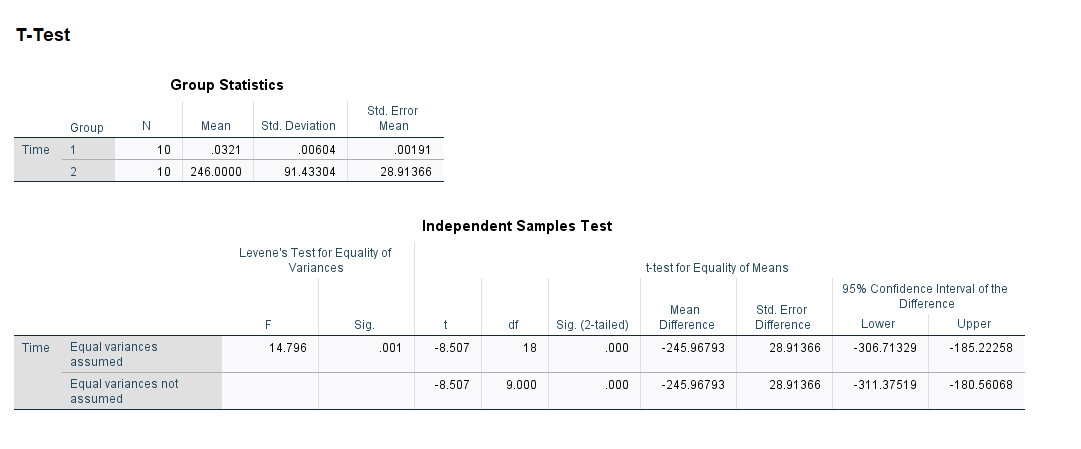
\includegraphics[width=15cm]{Images/ttest.png}
    \caption{Independent sample t-test}
    \label{fig:istt}
\end{figure}

The figure \ref{fig:istt} shows the results obtained by comparing the 
means of the time required by the automated system and medical professional to predict pigmented skin 
lesions. The group 1 in the test is reffered to the automated system and 
group 2 is reffered to medical professionals. Based on the p value obatined from the 
test which is 0.000 as in \ref{fig:istt} in the Sig(2-tailed) the null 
hypothesis is failed. Thus, it can be concluded that there is a significant 
difference in time required to peform diagnosis. The purposed automated machine 
is more time efficient to predict.

\section{Confusion Matrix}